\documentclass{aastex63}

%% Define new commands here
\newcommand\latex{La\TeX}
\graphicspath{{./}{figures/}}
\usepackage{graphicx}
\usepackage[most]{tcolorbox}
\usepackage{listings}
\providecommand{\keywords}[1]{\textbf{\textit{Index terms---}} #1}
\usepackage{caption}
\usepackage{subcaption}

\begin{document}

\title{The MW-M31 Dark Matter Merger Remnant 3D Distribution\\}

\author{Cassandra Bodin}
\affiliation{University of Arizona}

\keywords{Dark Matter Halo, 3D Distribution, Major Merger, Merger Remnant, Local Group, Milky Way, Andromeda}

%% Abstract
%%Sentence defining topic
%%Sentence as to why important
%%Sentence about question exploring
%%Each Finding --> What did you find?
%%Concluding Sentence

\begin{abstract}
In this paper I will study the evolution of the shape of the dark matter halo of the Milky Way and Andromeda galaxies before, during and after their merging event. By analyzing these dark matter distributions one can further understand the evolutionary path of not only our galaxy but also other galaxies with similarly shapes halos. The first step in this evolutionary understanding is to analyze the upcoming merger of two galaxies, of the Milky Way and Andromeda, in which we know all the kinematic and orbital dynamics. Knowing these features allowed astronomers to create a simulation data that modelled the merger. I used this data to model the 3 dimensional distribution of dark matter particles, resulting in initial spherical distributions for both galaxies, a triaxial ellipsoid distribution for a snapshot of the galaxies during the merger, and finally I found that the post merger distribution was a different triaxial ellipsoid. As a result of this data, I can conclude that a merging event alters the shape of the dark matter halos of the original host galaxies; and thus will greatly effect the evolution of the merger remnant through processes such as accretion, star formation, and orbital dynamics with other galaxies.
\end{abstract}


%% Start the main body of the article. If no sections in the 
%% research note leave the \section call blank to make the title.

%%Introduction
\section{Introduction} 

%%Define the proposed topic: 
%%MW/M31 Merger Remnant- Dark Matter Halo Evolution
%%Question: Is the 3D dark matter distribution spheroidal? or elongated like an ellipsoid.

Our universe consists of countless numbers of galaxies, each belonging to different subgroups. Our galaxy, the Milky Way (MW) belongs to a small subsection of galaxies that we call the local group. Within our local group the 3 largest galaxies, or dominant galaxies, are the MW, the Andromeda Galaxy (M31), and the Triangulum galaxy (M33). In 2012, using data from the Hubble Space Telescope, it was discovered that M31 is on a direct collision course for the MW, see Figure 1. The collision is projected to take place in approximately 4 billion years. \cite{Dunbar_2012} Throughout the time of the merger a substantial amount of changes will take place that will shape the evolutionary path of not only the MW but the entire local group. One such change will be the 3D distribution of dark matter. Currently the distribution has two main peaks centered on the MW and on M31. After the merger the two dark matter halos will coalesce, resulting in a single much larger peak in the dark matter distribution.

\begin{figure}[ht!]
\begin{center}
\includegraphics[scale=0.30,angle=0]{CollisionScenario.jpg}
\caption{\label{fig:1}, A depiction of the collisional path of the MW and M31 galaxies.  (Credit: NASA; ESA; A. Feild and R. van der Marel, STScI) \url{https://www.nasa.gov/mission_pages/hubble/science/milky-way-collide.html} }
\end{center}
\end{figure}

%%State why the topic matters to understanding our galaxy:
Understanding the outcomes of this merger is important when it comes to understanding the formation and evolution of galaxies, not just for our own but many others. For example in the early forming stages of the MW there was a major merging event with another galaxy, Gaia-Enceladus. This merger greatly affected the evolution of our galaxy, changing not only the internal structure of the MW but also affecting the dark matter distribution within the galaxy's halo.\cite{Helmi_2018} Because dark matter is the predominant source of mass within our universe, the 3D dark matter distribution within the halo of a galaxy directly links to how that galaxy evolves. The distribution will affect a galaxy's internal evolution. Dark matter halo growth depends on the potential well of the galaxy, thus a larger halo will accrete more gas and will retain more gas in the outflows. As a result of the increase in the amount of gas within the galaxy, more new stars will be able to form, increasing the size of the galaxy and causing alterations to the internal structure of the galaxy over time. Another effect of the 3D distribution of dark matter is how that galaxy interacts with other galaxies within the local group through orbital dynamics.\cite{Wechsler_2018} Therefore, being able to predict what will happen to the dark matter after the MW-M31 merger is an important part of being able to predict how our galaxy will evolve after the merger.

%%Overview of current understanding of the topic: 

The shape of the dark matter halo after the merger is completely dependent upon the initial conditions of the two galaxies before they merger, specifically in relation to their mass, angular momentum and other orbital properties, and energy of the merger. When analyzing the mass distributions of the halos via simulations Drakos et al.\cite{Drakos_2019} found that low energy mergers resulted in mass moving inwards towards higher density, whereas for high energy mergers the halo was more extended. Therefore, if we know the motions of the galaxies before and during the merger we should be able to speculate on the general shape of the dark matter halo, whether it be extended from the merger or not. Based on motions of both the MW and M31’s satellites, astronomers have created models for the shapes of the MW and M31’s dark matter halos pre-merger. The MW’s dark matter halo (see Figure 2) is modeled as a triaxial ellipsoid, or an ellipsoid where the radius along each axis (x,y,z) has different lengths. This discovery was made through the creation of models using the data for tidal debris the Sagittarius Dwarf Galaxy, a satellite of the MW. This data was obtained through digital sky surveys such as Two-Micron All Sky Survey and the Sloan Digital Sky Survey. \cite{Law_2010} Unlike the MW, M31’s modeled dark matter halo is a prolate spheroid, or a sphere that is elongated along the z axis, where the x and y axes are equal. This model of M31’s halo was created by Hayashi and Chiba \cite{Hayashi_2014} using nonspherical mass models of M31 and the positions of its satellites, and was compared with cold dark matter models. 

\begin{figure}[ht!]
\begin{center}
\includegraphics[scale=0.15,angle=0]{milky-way-triaxial-dark-halo.jpg}
\caption{\label{fig:2} A depiction of the triaxial shape of the MW halo, colored like a beach ball. The spiral in the center is the galaxy, white axes drawn for reference. Credit: David Law, UCLA \url{https://astronomy.com/news/2010/01/astronomers-map-the-shape-of-galactic-dark-matter} }
\end{center}
\end{figure}


%%What are the open questions in the field: define prolate,oblate,or triaxial halos
%%Prolate- elongated spheroids
%%Oblate- flattened spheroids
%%Triaxial- ellipsoids

One of the main questions regarding the distribution of dark matter post merger, is what the shape of the distribution will be. There are several different possibilities for these shapes, the two main being spheroidal or ellipsoidal. Within these two types of distributions there are other classifications to describe the shape of dark matter halos; prolate, oblate, and triaxial (see Figure 3). Prolate and oblate shapes are both spheroidal in shape, meaning they are both quadric surfaces that can be obtained by rotating an ellipse about one of its principal axes. Prolate describes a sphere that has been elongated into a football like shape. Oblate describes a sphere that has been flattened into a lentil like shape. Both these shapes follow the equation \(\frac{x^2 + y^2}{a^2} +\frac{z^2}{c} = 1\), where a is the semi-axis and is also the equatorial radius of the spheroid, and c is the distance from the center to the edge along the symmetry axis. If $c>a$ then it is a prolate spheroid, if $c<a$ then it is an oblate spheroid, and if $c=a$ it is an exact sphere. The halo would be triaxial if it were ellipsoidal and each of the 3 axes had a different length. This would follow the equation \(\frac{x^2 }{a^2} +\frac{y^2 }{b^2}+\frac{z^2}{c} = 1\), where a is the semi-major axis, b the semi-minor axis and c is the distance from the center to the edge along the symmetry axis; and $a \neq b \neq c$. \cite{Bovy_2017} The MW- M31 merger should result in a dark matter halo with one of these shapes.

\begin{figure}[ht!]
\begin{center}
\includegraphics[scale=0.20,angle=0]{halotypes.png}
\caption{\label{fig:3}A model of the different types of dark matter distributions in galactic halos (prolate,oblate,or triaxial halos) from section 13 of the article Dynamics and Astrophysics of Galaxies, \url{http://astro.utoronto.ca/~bovy/AST1420/notes/notebooks/III-01.-Triaxial-Mass-Distributions.html} }
\end{center}
\end{figure}


%%This Project
\section{The Project} 

%%Specific Questions: Is the 3D dark matter distribution spheroidal, or elongated like an ellipsoid? How does the shape affect future evolution?

In this paper I will be studying how the 3D dark matter halo distribution changes as the MW and M31 galaxies undergo collision and after the merger. Before the merger the MW and M31 dark matter halos are modeled to be roughly spherical for the purposes of the data I will be using. As the galaxies merge the dark matter halos of both galaxies will also collide and the distribution of dark matter around the resulting merger remnant will be different from that of the initial shapes. I will be focusing on finding out what that shape will be, be it a triaxial ellipsoid, an oblate spheroid, or a prolate spheroid.  I will be using code to model and plot simulated data of the merger in order to visualize and accurately represent the distributions.

%%What is the open question?%%Why is this important for understanding galaxy evolution?
The distributions of dark matter particles in the halo will change throughout the merger as the different particle types interact with each other. By utilizing the model data and python code I will be able to determine the shape of the 3D dark matter distribution throughout the merger, spheroidal or ellipsoidal. From this data I will be able to draw conclusions based on the shapes that are found. 
The MW and M31 data is particularly special because we have all of kinematic and orbital information due to the proximity of the galaxies. Therefore we are able to create a very accurate model of what might happen in the future. By creating this model and understanding the kinematics involved in the merger astronomers will be able to make educated assumptions of how other galaxies will evolve due to collisions. We can take our own galaxy and use it to better understand the universe. 

%%Methodology
\section{Methodology}

%%Introduce the Coding Simulations (reference paper \cite{Marel_2012}, explain meaning of N-body simulation)
I will be using the MW-M31 collision data, provided by Professor Gurtina Besla, and code in python to study and model the 3D distribution of dark matter before, after, and during the MW-M31 merger; focusing on the distribution post-merger. The collision data has been used for another paper that analyzes the evolution of the MW, M31, and M33 orbital evolution throughout the merger, as well as the fate of our Sun by Van Der Marel et al. \cite{Marel_2012} The data is an N-body simulation, meaning a large number of particles of different types were generated around an object, in this case the galaxies, that each interact with each other. Each particle’s motion will be affected by the dynamics of every other particle in the system. Thus, the interactions of the particles as they move over time will have to be taken into account throughout the code.

%%Overview of approach. What are you trying to do?
The code I am creating will model the positions of the dark matter particles at a given snapshot, take those positions and plot them in 3D, and will overplot shapes until a match can be identified. It will utilize other, pre-written programs to pull in the MW-M31 collision data from the specific files I have selected and will find the positions in space of the dark matter halo ‘particles’ by calculating the center of mass of each particle. In addition to these programs I will write pieces of code that will take in this data and plot it in 3D using a matplotlib subpackage called \lstinline{mpl_toolkits.mplot3D}. This package will allow me to not only plot in 3D, but also to choose the type of display for the data, such as contour plots, scatter plots, line plots, surface plots and more. I will also be using this code to plot a wire-frame shape over a scatter plot of the distribution of particles, in order to fit the shape to the distribution and identify if that shape is a triaxial ellipsoid, oblate spheroid, or prolate spheroid. I will do this for the distributions of dark matter particles for both the MW and M31 pre-merger, as well as, for the combined MW-M31 merger remnant. The final result should look something like the image in Figure 4, which shows the theoretical projected shape of the MW dark matter halo as it is currently, pre merger.

%%Figure (1+)
\begin{figure}[ht!]
\begin{center}
\includegraphics[scale=0.35,angle=0]{mergersnapshot_finalresulthypothesis.png}
\caption{\label{fig:4}This figure is a theoretical prediction of what my resulting plot of the shape of the dark matter halo may look like. The underlying image is a snapshot of the remnant from NASA’s Crash of the Titans: Milky Way and Andromeda Collision simulation video at  \url{https://svs.gsfc.nasa.gov/30955}}
\end{center}
\end{figure}

%% Describe the calculations the code will compute. Include all relevant eq. Describe code in Readfile.py, MassProfile.py, and CenterOfMass.py

I will be using pieces of my code in Lab7, which calls in other programs I wrote such as Readfile.py, MassProfile.py, and CenterOfMass.py to process the disk particles throughout the merger and display them in 2D density contour plots, to form a basis for my code. Readfile.py is a relatively simple program that reads in the position, velocity, and mass data for a specified file containing a ‘snapshot’ of the collision data. Having this program allows me to easily read in whatever file I want in a single line of code. It is used in each of the programs I will be using. MassProfile.py creates a series of mass profiles and rotation curves for a selected type of particle (halo, disk, or bulge). It contains several different types of mass profiles including the Hernquist 1990 Mass Profile and the Mass Enclosed within a radius of each of the particles. The Hernquist Mass Profile contains the most relevant information as it specifically deals with the profile for the dark matter halo. The equation for the Hernquist Mass Profile is \[M_{hern}= \frac{M_{halo}*R^2}{(R+a)^2}\qquad Eq1\]
Where $M_{hern}$ is the Hernquist Mass given in units of $M_\odot\ $, $M_{halo}$ is the mass of the halo particles in $M_\odot\ $ , R is the radius, in \si{kpc}, from the center of the galaxy that encloses the particles, and a is the scale length, also in \si{kpc}. The Mass Enclosed functions don’t have any special equations but instead just add up the mass of a particle type that is enclosed within a certain radius.MassProfile.py also used the mass profiles it created to generate rotation curves by calculating the circular velocity using the general equation \[V_{circ}= (\frac{G*M_{encl}}{R})^{1/2}\qquad Eq2\]
Where $V_{circ}$ is the circular velocity in $\frac{km}{s}$, G is the gravitational constant $G=4.498768e-6 kpc^3Gyr^{-2}M_\odot\ ^{-1}$, and $M_{encl}$ is the mass enclosed within a certain radius in $M_\odot\ $. This Program will likely be useful for finding out the values of the mass enclosed within our shape, which is not essential to our goal but is still useful information. 
The last program I will be using is the CenterOfMass.py program. This program calculates the center of mass positions (COMP) and velocities (COMV) for each snapshot of the data. It accepts the position data from the designated file and iterates to calculate the COMP for each of the particles relative to each other. Thereafter it calculates similarly the COMV considering the COMP it had just calculated. The COMP is what I will be using to identify where each particle is located in the 3D dark matter distribution. The last piece of my code will be a snippet to draw the shapes in 3D. These shapes will have to be coded in (see Code Snapshot) with arbitrary values for a, b, and c such that they fit the description of each of the shapes (triaxial, oblate, or prolate) and adjusted later to fit over the distribution of dark matter particles.
\newpage
\begin{tcolorbox}[breakable, enhanced]
Code Snapshot
\begin{verbatim}
#set up parameters for the shape we're fitting the 3D distribution to
u=np.linspace(0.0, 2.0*np.pi,60)
v=np.linspace(0.0, np.pi,60)

#normalization parameter (change to easier fit the size of the shape, begin with norm=1)
norm=1

#shape 1 Triaxial ellipsoid
coef1=(7,5,3)
rx1,ry1,rz1=norm/np.sqrt(coef1)
x1= rx1*np.outer(np.cos(u),np.sin(v)) #choose size for x
y1= ry1*np.outer(np.sin(u),np.sin(v)) #choose size for y
z1= rz1*np.outer(np.ones_like(u),np.cos(v)) #choose size for z

#shape 2 Prolate Spheroid
coef2=(10,10,1)
rx2,ry2,rz2=norm/np.sqrt(coef2)
x2= rx2*np.outer(np.cos(u),np.sin(v)) #choose size for x
y2= ry2*np.outer(np.sin(u),np.sin(v)) #choose size for y
z2= rz2*np.outer(np.ones_like(u),np.cos(v)) #choose size for z

#shape 3 Oblate Spheroid
coef3=(3,3,10)
rx3,ry3,rz3=norm/np.sqrt(coef3)
x3= rx3*np.outer(np.cos(u),np.sin(v)) #choose size for x
y3= ry3*np.outer(np.sin(u),np.sin(v)) #choose size for y
z3= rz3*np.outer(np.ones_like(u),np.cos(v)) #choose size for z
\end{verbatim}
\end{tcolorbox}

%%Describe the plots you will create. One can use code from the class the other has to be your own code
In order to visualize the 3 dimensional distribution of dark matter, my code must output a series of plots. Before I can begin plotting in 3 dimension I will plot contour plots in 2 dimensions along the major axial planes, XY, YZ, and XZ, in order to fit the parameters for a, b, and c the most closely. These fits will align as closely with a density contour that contains 99.99\% of all the dark matter particles. With this data I can move on to the 3 dimensional plots. The first set of 3 dimensional plots will depict the dark matter distribution of the MW and M31 before the merger. This set of plots will be generated to test if the code is working. The data I was given assumes that initially the dark matter halos are roughly spherical, so the distribution in this plot should also be spherical. The next plots will be a snapshot of a distribution during the merger. I added this plot in order to better visualize what was happening between the beginning of the merger and the end. The next part of the code will output the dark matter distribution of both the MW and M31 after the merger on the same graph. For each of these plots I added a section of code that will make the background black, \lstinline{ax.set_facecolor('black')}, and I made the stars either white (for the MW) and light blue (for M31). I also added another snippet of code that can allow you to change the orientation of the 3D plot, so you can view the distribution from above, below, at an angle and face on using \lstinline{ax.view_init(A,B)} where A and B are angles of rotation. All of these additions were made to better be able to visualize and analyze the distribution. After creating all of these plots I will overplot the shape options and adjust the parameters (see Code Snapshot) to fit the shape of the distribution. Once I find which one fits the best, I will find my final result on which shape the 3D dark matter halo distribution follows.

%%What is your hypothesis on what you'll find? Why?
Based upon the current models of the shapes of the halos of MW, as triaxial \cite{Law_2010}, and M31, as prolate \cite{Hayashi_2014}, thus I would hypothesize that the resultant merger halo will be a  triaxial ellipsoid. Assuming that the dark matter halos of each galaxy do not completely change during the merger, then the combined halo of the remnant could theoretically be similar to the shape if you added both of the halos together. Adding a prolate object to a triaxial object would result in a triaxial object. However, the simulation data assumes that both the MW and the M31 halos are roughly spherical, which will alter the shape of the post-merger halo. Even though, as a result, the shape might be a little harder to distinguish I still would hypothesize that it still would be a triaxial ellipsoid, though it will probably be relatively close to spherical with only slight variations in a, b, and c. I would hypothesize this because the MW has already undergone a merging event with Gaia-Enceladus \cite{Helmi_2018}, and thus its dark matter distribution is the result of a merger already. Therefore, it is very likely that the result of another merger will be a triaxial ellipsoid as well.

\section{Results}

%%2D distribution fitting graphs
\begin{figure}[ht!]
\centering
\begin{subfigure}{0.3\textwidth}
\centering
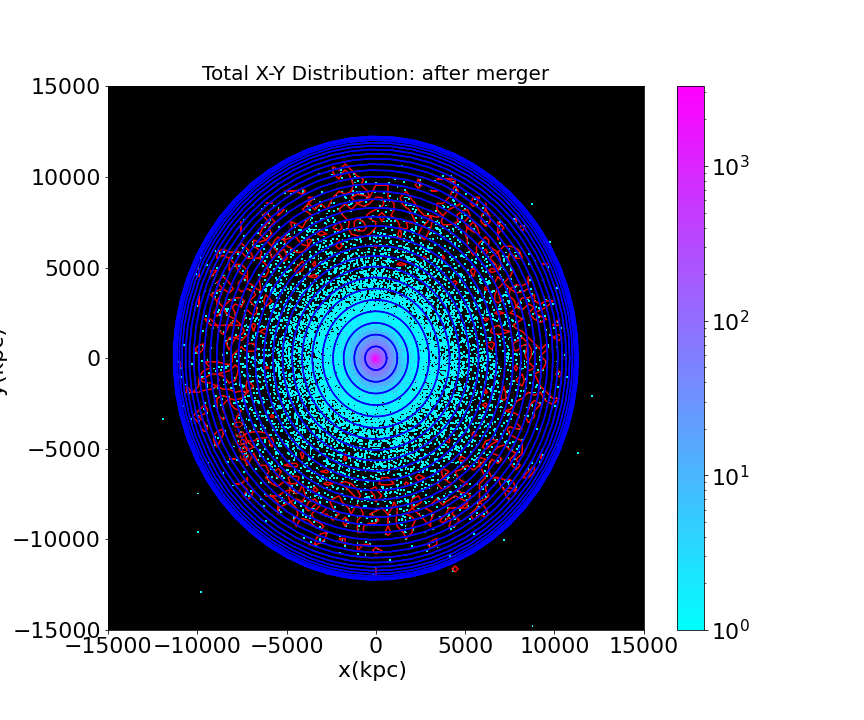
\includegraphics[width=\linewidth]{XY_Halo_a_Total.png}
\caption{\label{fig:5a}}
\end{subfigure}
\begin{subfigure}{0.3\textwidth}
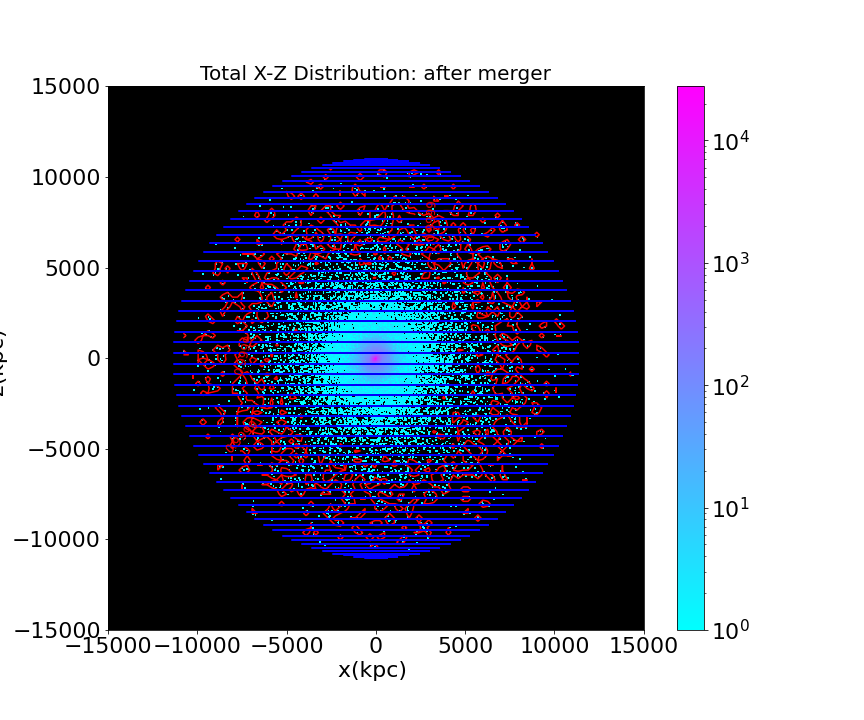
\includegraphics[width=\linewidth]{XZ_Halo_a_Total.png}
\caption{\label{fig:5b}}
\end{subfigure}
\begin{subfigure}{0.3\textwidth}
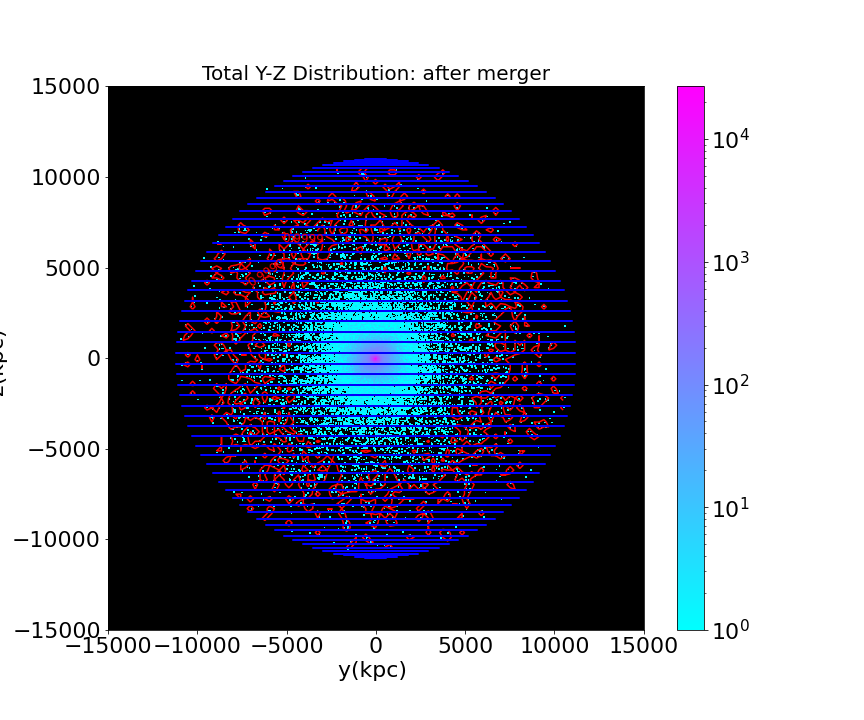
\includegraphics[width=\linewidth]{YZ_Halo_a_Total.png}
\caption{\label{fig:5c}}
\end{subfigure}
\caption{The above are 2D density distributions of dark matter halo particles for the merger remnant along the a) XY, b) XZ, and c) YZ planes respectively. The underlying colors from light blue to pink represent the density of dark matter particles. The red lines depict a contour in the density that contains 99.99\% of the particles. The blue is the 3D shape generated in a 2D depiction in order to identify the approximate values of a, b, and c; which will be used to determine the shape of the final distribution.
Note: Other distributions were also generated for: M31 pre-merger, MW pre-merger, and the merger.}
\centering
\end{figure}

%%Analyze Result 1
The first result I had from my code showed the three different 2D distributions for both MW and M31 before the merger and the combined after the merger. Using the contour code in Lab7, I matched the parameters for a, b, and c to the density contour that held 99.99\% of the distribution. By creating these plots I could construct a better fit for my final code creating 3D distributions of dark matter particles. I used the pre-merger data in order to test the code, as both the MW and M31 distributions before the merger were approximated to be completely spherical. Examples of the output of this code can be seen in Figure 5, which depicts the 2D density distributions of the merger remnant. 
\vspace{4mm}
\begin{table}[h!]
\begin{tabular}{| c | c | c | c | c |}
 \hline
  & M31 Before Merger  & MW Before Merger & Total During Merger & Total After Merger \\ 
 \hline\hline
 $a_{norm}$ & 1.95 & 1.9 & 1.8 & 1.75 \\ 
 \hline
 $b_{norm}$ & 1.95 & 1.9 & 1.7 & 1.8 \\
 \hline
 $c_{norm}$ & 1.95 & 1.9 & 1.9 & 1.85 \\
 \hline
 a (kpc) & 10741.723 & 10882.144 & 1180.340 & 1136.934 \\ 
 \hline
 b (kpc) & 10741.723 & 10882.144 & 11504.475 & 1180.340 \\
 \hline
 c (kpc) & 10741.723 & 10882.144 & 10882.144 & 0.196 \\
 \hline
\end{tabular}
\caption{This table holds all of the values for a, b, and c for each of the galaxy distributions. $a_{norm}$, $b_{norm}$, and $c_{norm}$ correspond to the values found using a normalisation factor of 15000. a, b, and c are the true values in kpc, which were generated by the code for each galaxy distribution.}
\end{table}

For the initial 2D plots, examples shown in Figure 5, I used a normalization parameter of $norm=15000$. This allowed me to vary relatively small numbers in order to fit the plots precisely instead of guessing completely at the high numbers. Thus the results using the normalization parameter were as shown in Table 1 as $a_{norm}$, $b_{norm}$, and $c_{norm}$. Later In the code when I generated the 3D plots (see Figure 6), I wrote a piece of code that also output the true values which are labeled a, b, and c in Table 1. These values agree with the theory that the dark matter halo radius is somewhere between 5-7 times the virial radius of the galaxy\cite{Prada_2006}, which for the milky way is approximately 200kpc. The MW and M31 are similar in size, thus I would expect that their dark matter halos are also similar in size. Therefore, I would expect all of these values to be somewhere between 10,000kpc and 14,000kpc. 

For M31 before the merger all of the normalized values were the same; and thus all of the true values were also all the same. The resulting distribution was then proven to be spherical. Likewise, the MW pre-merger 3D distribution was also found to be spherical. Although the M31 and MW dark matter halo particle distributions were found to be spherical, both the distributions for during and after the merger were not. As shown in Table 1, the values found for a, b, and c were not equal, in fact $a\neq b \neq c$. This inequality between each of the values means that this distribution is a triaxial ellipsoid. The final distribution also has unequal values of a, b, and c, leading to the conclusion that the final distribution is also a triaxial ellipsoid. Despite these last two distributions being triaxial, they are not equal. Their values of a, b, and c are different, showing that the galaxies changed shape over time as they underwent the merger. 

%3D before, during, and after distributions 
\begin{figure}[h]
\centering
\begin{subfigure}{0.35\textwidth}
\centering
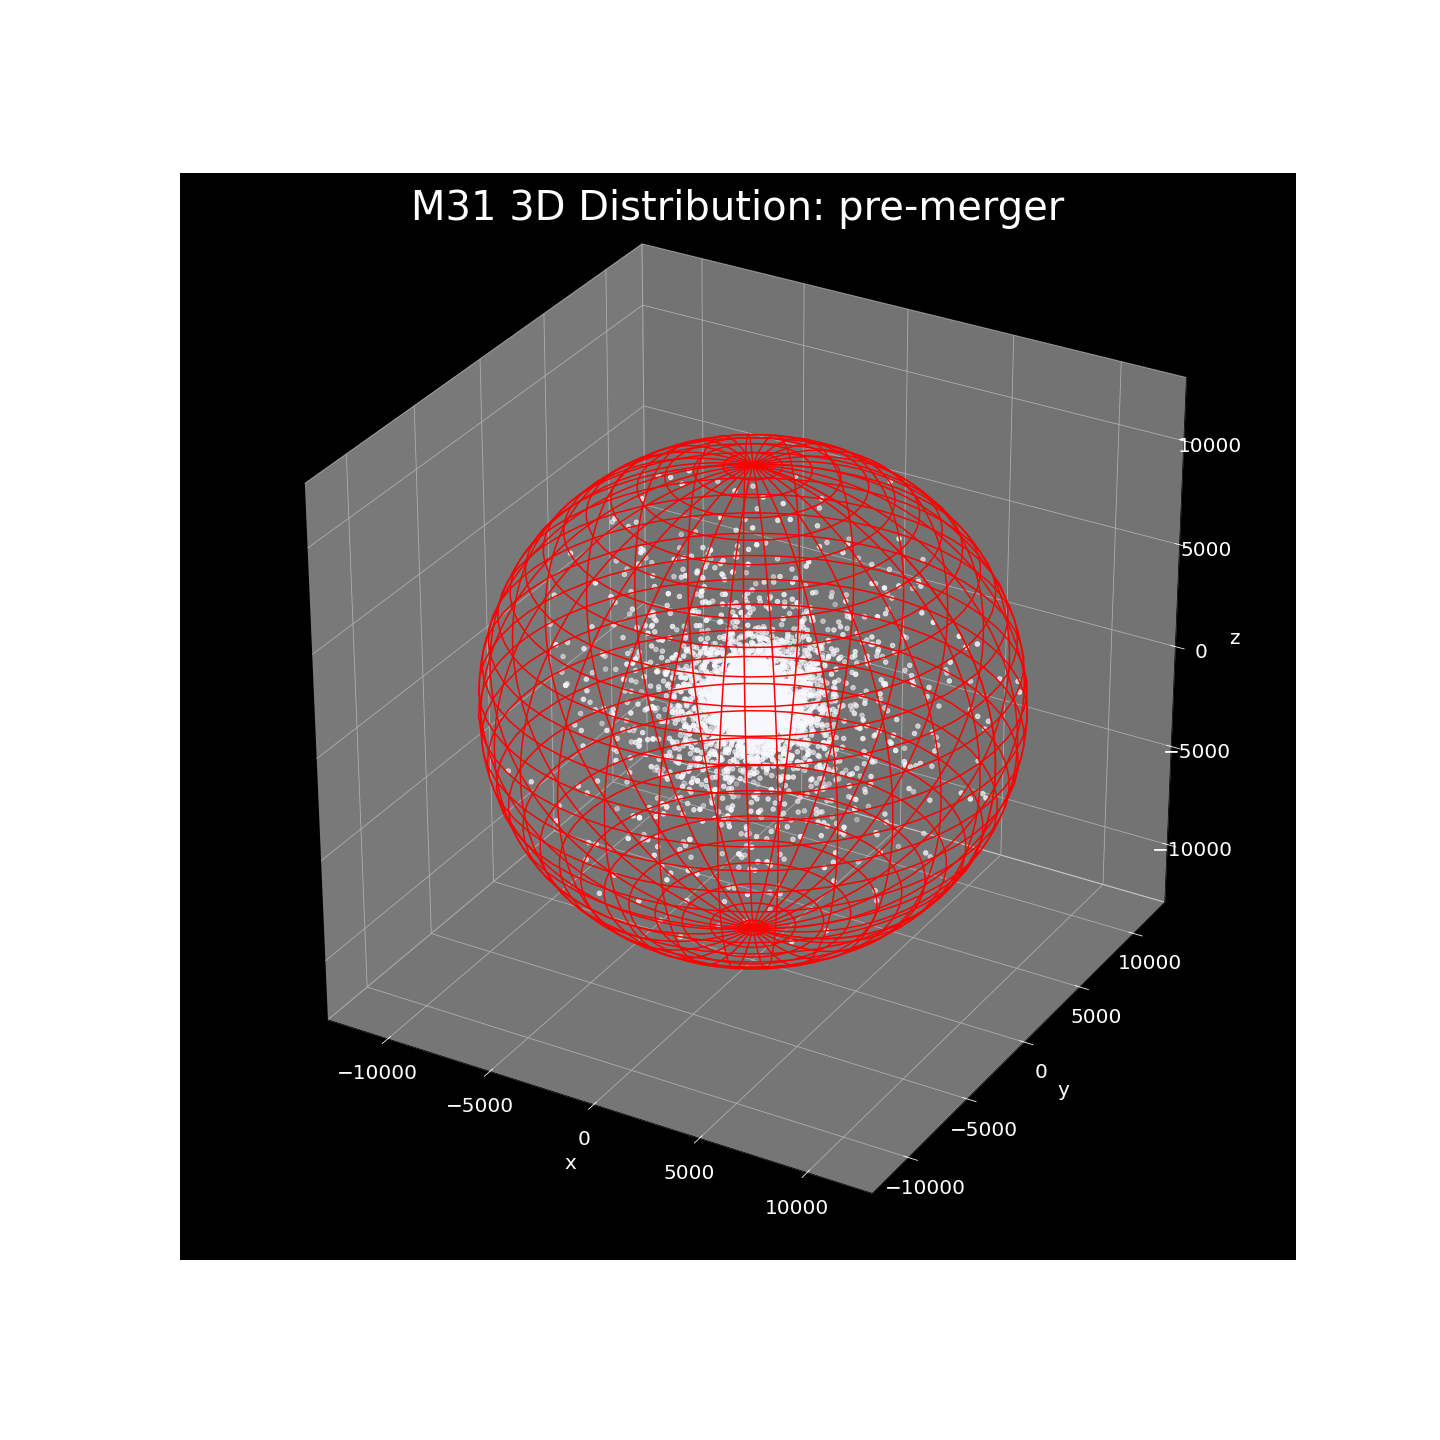
\includegraphics[width=\linewidth]{M31_bmerge.png}
\caption{\label{fig:6a}}
\end{subfigure}
\begin{subfigure}{0.35\textwidth}
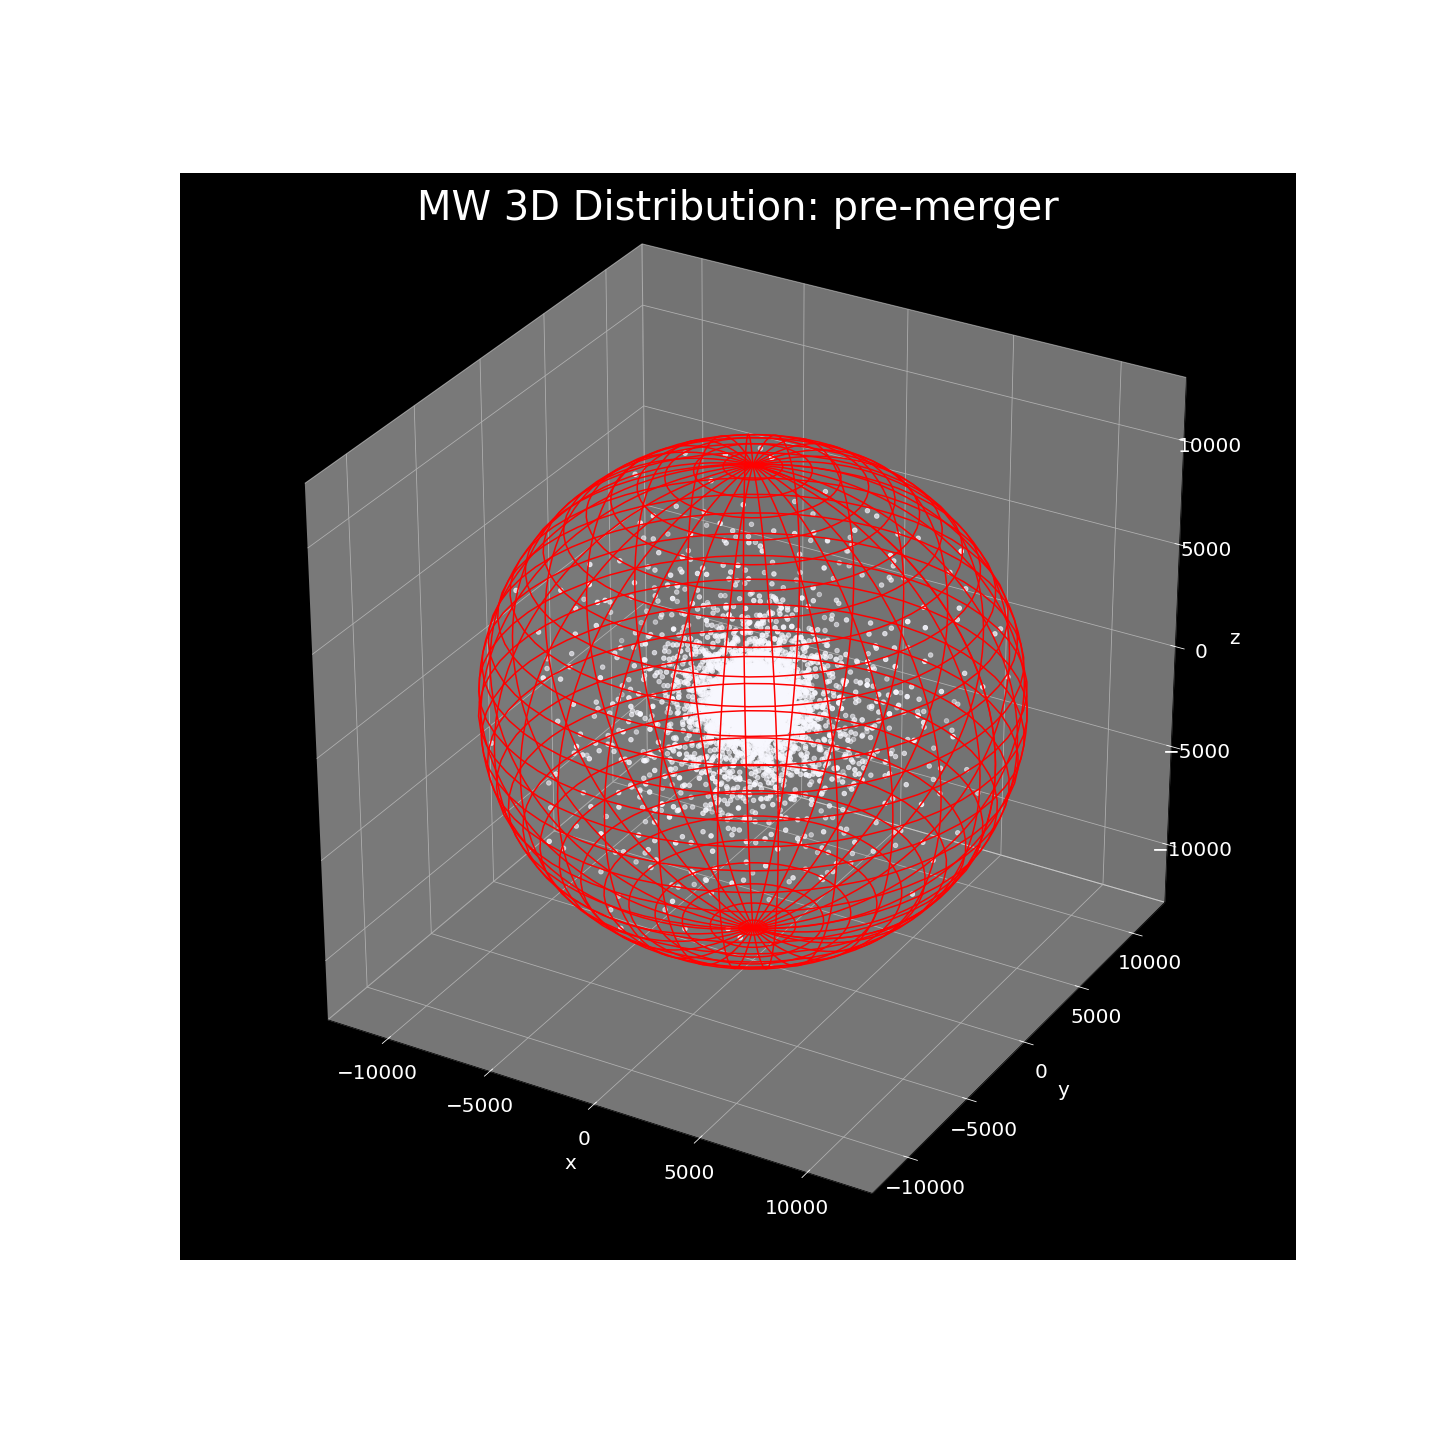
\includegraphics[width=\linewidth]{MW_bmerge.png}
\caption{\label{fig:6b}}
\end{subfigure}
\begin{subfigure}{0.35\textwidth}
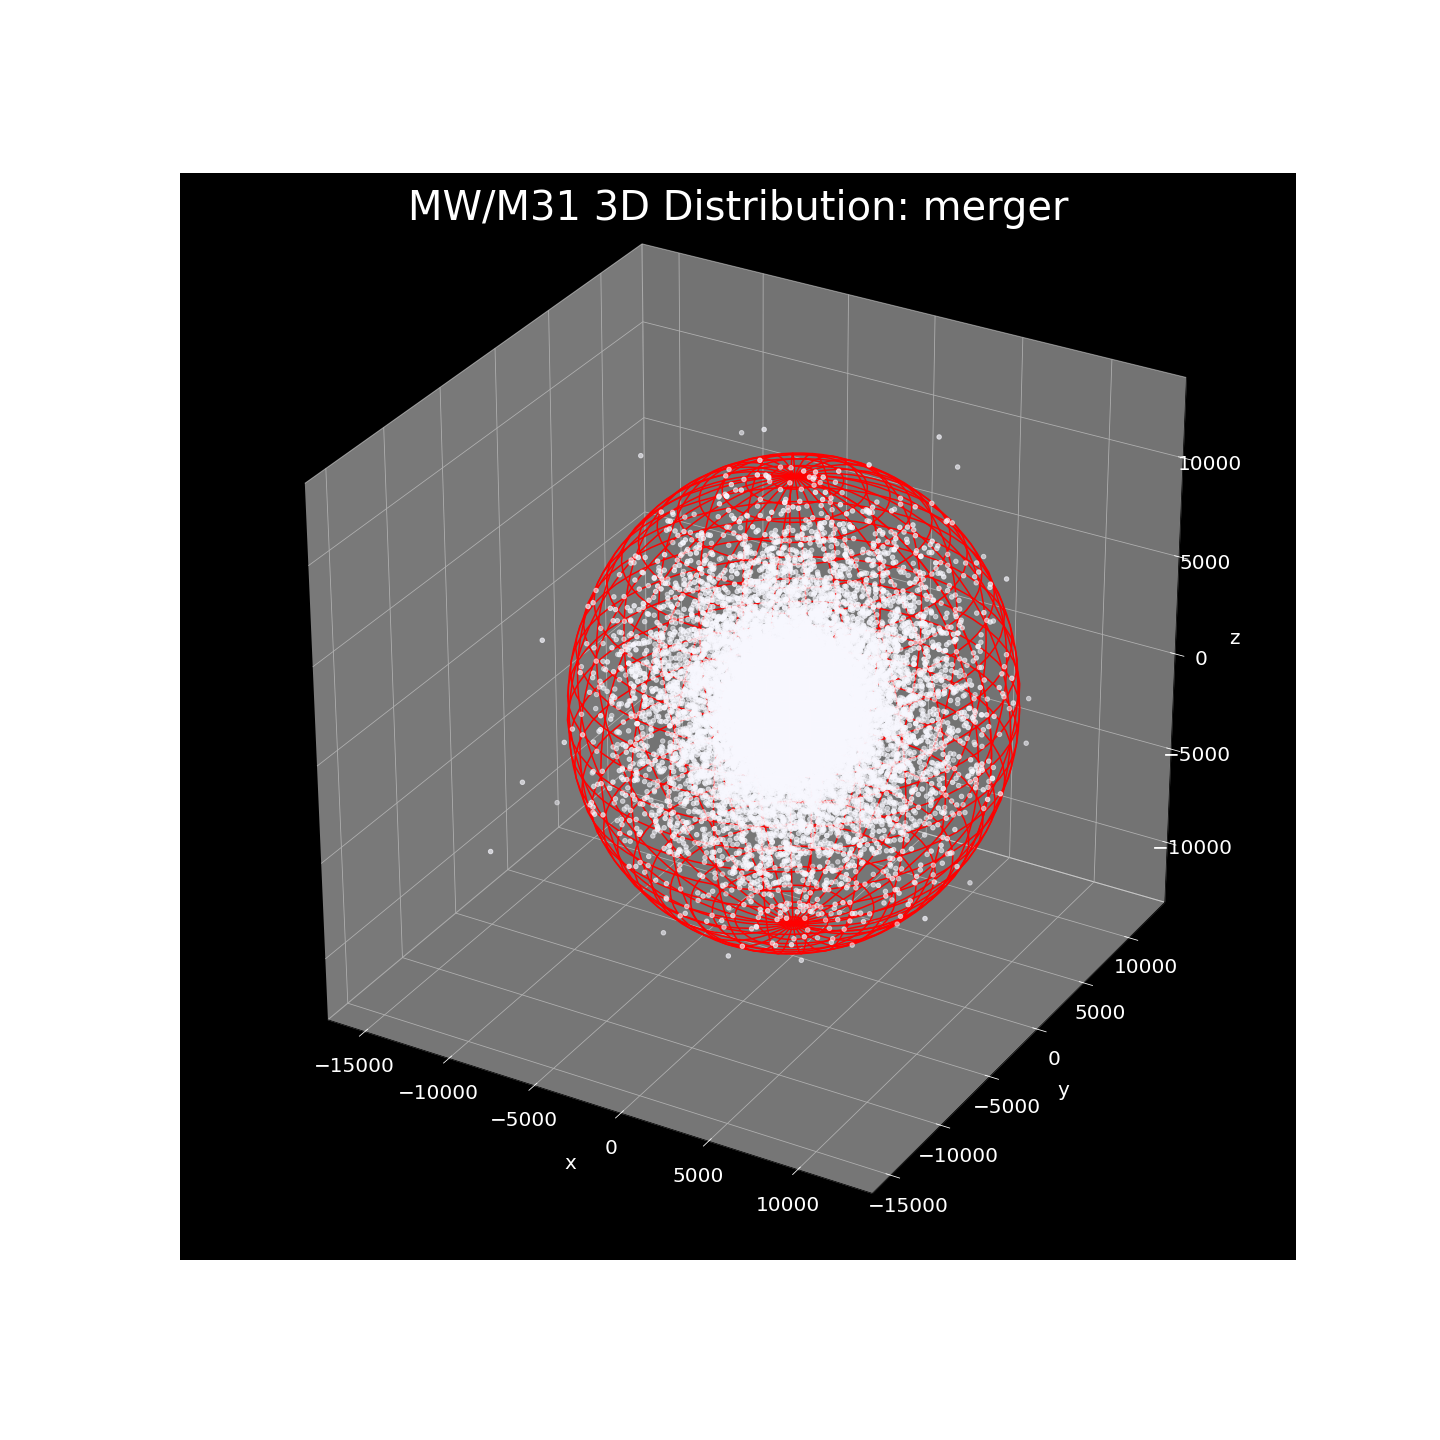
\includegraphics[width=\linewidth]{M31MW_dmerge.png}
\caption{\label{fig:6c}}
\end{subfigure}
\begin{subfigure}{0.35\textwidth}
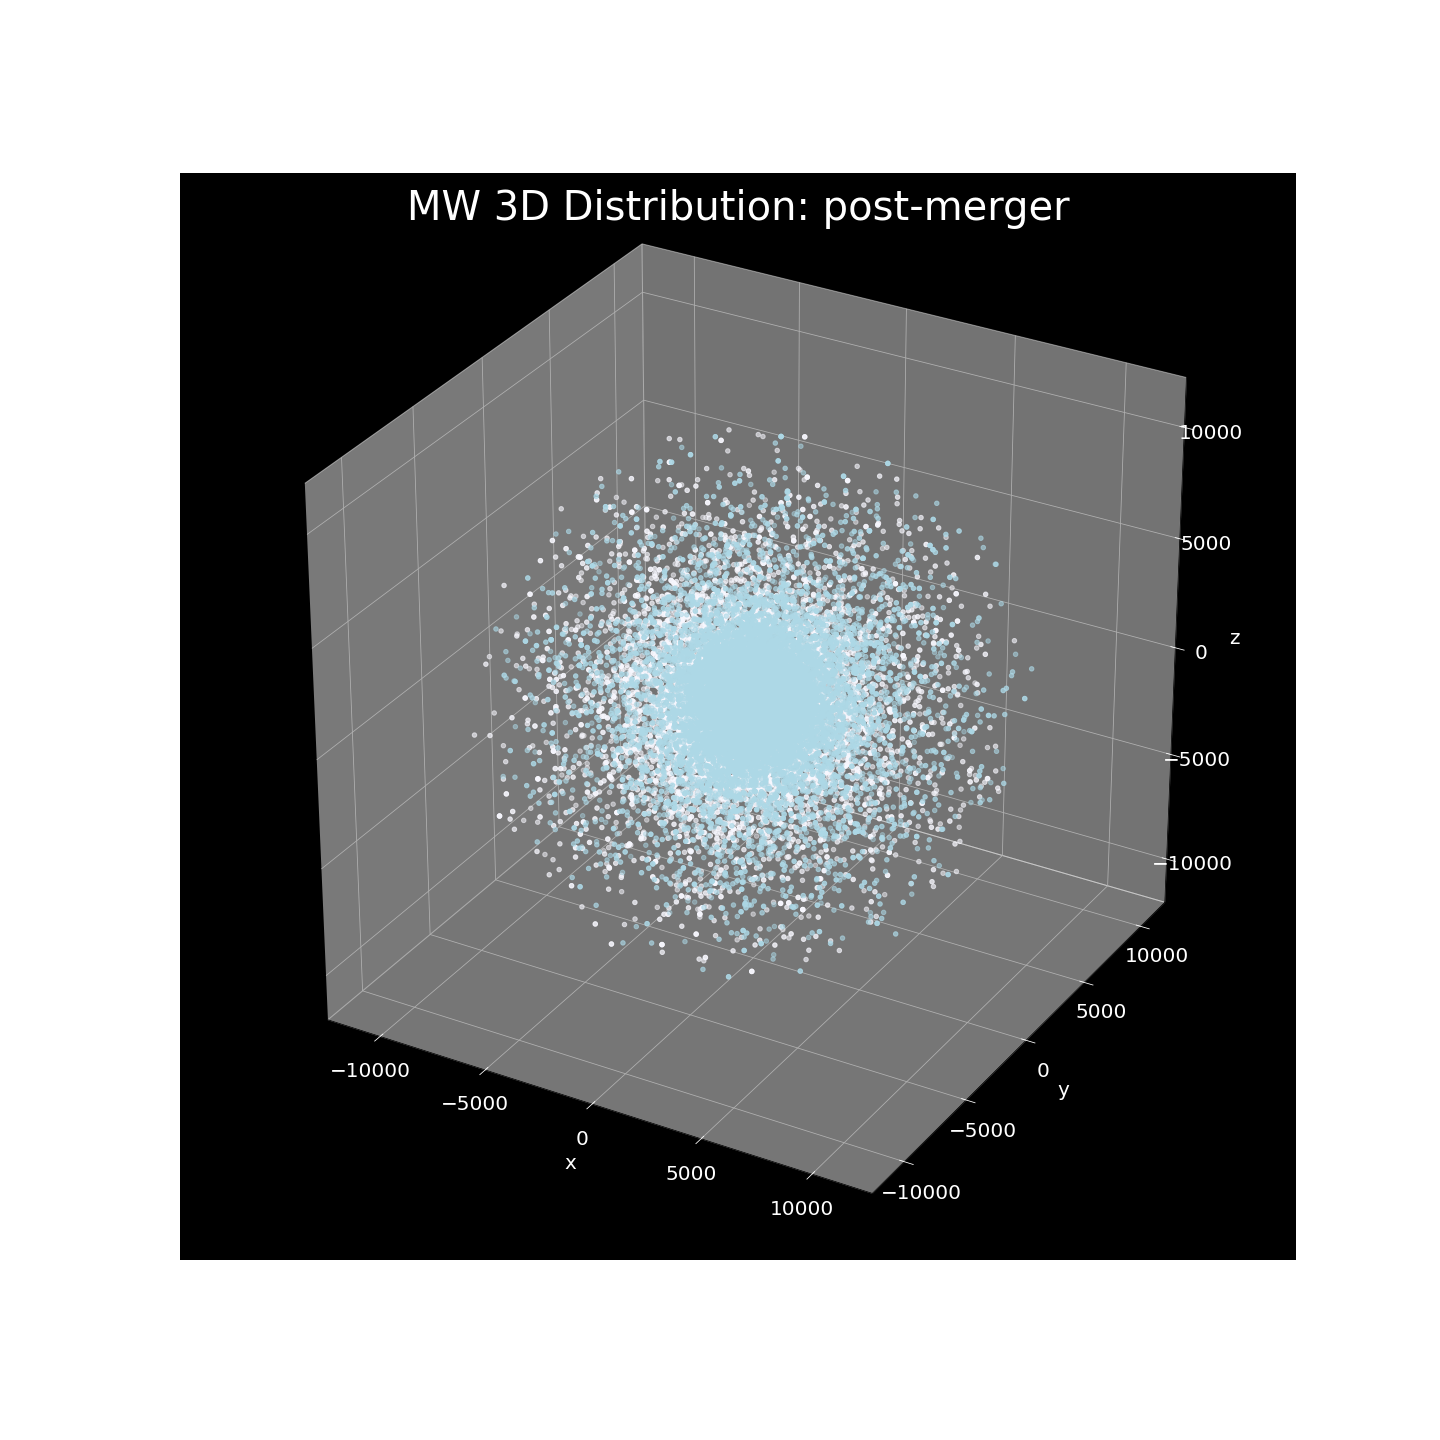
\includegraphics[width=\linewidth]{M31MW_amerge.png}
\caption{\label{fig:6d}}
\end{subfigure}
\caption{The above figures are 3D distributions of dark matter halo particles evaluated such that 99.99\% of particles lie within the wire-frame shape. a) The distribution of M31 before the merger. b) The distribution of MW before the merger. c) The total distribution of both galaxies during the merger. And d ) The total distribution of both galaxies after the merger.}

\end{figure}
The results shown in Figure 6 are the actual 3D dark matter halo distributions for before, during, and after the merger. I used the results in Table 1, found using graphs such as those shown in Figure 5, for the values $a_{norm}$, $b_{norm}$, $c_{norm}$, and the normalization parameter in my final code to generate the wire-frame shape of each of the distributions. Using this code we found that the results in the above paragraph regarding the shapes of each distribution were correct. Both of the pre-merger 3D distributions were spherical (see Figures 6a and 6b). The distribution during the merger was triaxial at the snapshot that I chose, Snapshot 400/801 (Figure 6c). The final merger remnant distribution was also triaxial (Figure 6d) though which values of a, b, and c were the biggest to smallest were different from that of the distribution during the merger. For the distribution during the merger the order was as follows $c<a<b$; whereas after the merger remnant the order was $c<b<a$. This secondarily proves that not only does the merger cause the dark matter distribution to become triaxial but also that the merger was changing over time in between the initial merging event and when the merger was over.



\section{Discussion}
%%Summarize Results (1 paragraph per)
%%Does it agree with the hypothesis?
%%Does it relate to current literature?
%%What is the importance of this result?
Overall, I was able to generate a series of 3D plots representing the distributions of dark matter halo particles at different points during the merger, by first utilizing 2D plots along the different x, y, z planes in order to find the parameters for the wire-frame shapes in Figure 6. The first two figures, a and b, show the distribution for the galaxies before the merger occurred. This gave me insight into whether or not the code was working, as I knew that the simulation data initially modeled the halos as spheres. The third figure, c, depicts a snapshot of the distribution during the merger so I could see an evolution from the initial distributions to the final distribution. The final distribution, Figure 6d, I found to be a triaxial ellipsoid. This last result answers the big question of this paper; what is the shape of the final 3D distribution of the dark matter particles for the post merger remnant? The answer is a triaxial ellipsoid, where each of the three axis, a, b, and c, are unequal. This result fits with my hypothesis earlier on that the distribution should be triaxial, based upon what the non-simulation projection of the MW's dark matter halo currently is. The MW's dark matter halo in reality is slightly triaxial\cite{Law_2010} due to a previous merger event with the Gaia-Enceladus Galaxy. Thus, it seems that as two galaxies collide their interactions throughout the merger will result in a triaxial ellipsoid halo. Understanding how the dark matter halos evolve over time throughout merging events, such as this, is important in understanding galaxy evolution overall, due to the interactions between dark matter and other particle types within a galaxy.

\section{Conclusion}
%%Summarize intro (Q1-4) of abstract
    %%Sentence defining topic
    %%Sentence as to why important
    %%Sentence about question exploring
%%Highlight a key finding --> what does it mean? agree with hypothesis?
%%Future Directions --> where could this go? What could I do to go further? Improvements could make to code?
In order to understand our universe, how it began and what it will become, we must first look at how different pieces of the universe interact with each other. One such interaction is the collision and merger of galaxies that we have information on. The MW and M31 merger is an ideal event to model in order to understand more about our universe, as it is one of the most accurate models we can create because it is "close to home" so to speak, and we have all of the information on their orbital and kinematic motion. Using this modeled data, I was able to analyze and model the shape of the dark matter halo as the two galaxies underwent a merging event. The initial distributions before the merger were roughly spherical and the final distribution of the merger remnant was a triaxial ellipsoid. This result agreed with my hypothesis that was based on the Gaia-Enceladus/MW merger, which in reality caused the MW's dark matter halo distribution to be slightly triaxially ellipsoidal in shape, unlike the assumed spheroidal distribution in the simulation data. Thus, this would imply that theoretically any merging event would likely result in a triaxial shaped dark matter halo. If this is true and can be proven with the analysis of different merging events, then we would know more about how galaxies have and will evolve in the future. All of this will have to be explored further in order to make any definitive claims. If I were to continue this project I would attempt to map the distributions for all the data and attempt to piece together a collective mp4 file containing the animated evolution of the distribution from before the merger until the end. I would also have liked to use data modelling the initial dark matter halos as being more accurate in shape, the MW as a triaxial ellipsoid and M31 as a prolate spheroid, rather than a spherical distribution in order to see the differences in the final results. There is always more data to collect and analyze, and always more to learn about our universe.

\section*{Acknowledgement}
I am grateful to Professor Gurtina Besla and Rixin Li for not only contributing the data that made this project possible but also for making suggestions and assisting me when I was stuck with my code. I also wish to show my gratitude to all those who created the software packages that were used in my code, such as the authors and creators of Astropy\cite{Astropy Collaboration_2018}, matplotlib\cite{Hunter_2007}, numpy\cite{Van Der Walt_2011}, scipy\cite{SciPy_2020}, and ipython\cite{Perez_2007}. Without all of you this project would not have been possible.




%%Cited Journal Papers (3+)
%%\cite{Dunbar_2012} #NASA Hubble Space Discovery of collision M31-MW
%%\cite{Helmi_2018} #Gaia-Enceladus MW merger
%%\cite{Wechsler_2018} #dark matter halo- galaxy evolution
%%\cite{Drakos_2019} #current understanding of DM Halo predictions
%%\cite{Law_2010} #Astronomers map DM, triaxial MW halo
%%\cite{Hayashi_2014} #prolate halo of M31
%%\cite{Bovy_2017} #prolate,oblate,or triaxial halos

%%Cited programs
%%\cite{Astropy Collaboration_2018} #astropy
%%\cite{Hunter_2007} #matplotlib
%%\cite{Perez_2007} #IPython
%%\cite{SciPy_2020} #scipy
%%\cite{Van Der Walt_2011} #numpy


%%Other citations that might possibly be useful later
%%\cite{Cox_2008} #collision MW-Andromeda 
%%\cite{Dubinski_2008} #visualizing N body systems, DM for MW-M31 and local group vs Virgo
%%\cite{Garner_2017} #shining light on DM
%%\cite{Hayashi_2014} #prolate halo of M31
%%\cite{Hoffman_2007} # future of local structures DM and DE
%%\cite{Marel_2012} # MW M31 M33 evolution, merger, fate of sun
%%\cite{Prada_2006} # how far does a dark matter halo extend

\begin{thebibliography}{}

\bibitem{Dunbar_2012} Dunbar, Brian and Garner, Robert \ 2012, NASA

\bibitem{Helmi_2018} Helmi, Amina and Babusiaux, Carine and Koppelman, Helmer H. and Massari, Davide and Veljanoski, Jovan and Brown, Anthony G. A.\  2018, Nature, 563,7729, 85–88

\bibitem{Wechsler_2018} Wechsler, Risa H. and Tinker, Jeremy L.\  2016, Annual Review of Astronomy and Astrophysics, 56, 1, 435-487 

\bibitem{Drakos_2019} Drakos, Nicole E. and Taylor, James E. and Berrouet, Anael and Robotham, Aaron S.~G. and Power, Chris \ 2019, mnras, 487,1,993-1007

\bibitem{Law_2010} Law, David \ 2010, Astronomy.com

\bibitem{Hayashi_2014} Hayashi, Kohei and Chiba, Masashi \ 2014, APJ,789,1,62

\bibitem{Bovy_2017} Bovy, Jo \  2017, Dynamics and Astrophysics of Galaxies, 13

\bibitem{Marel_2012} Marel, Roeland P. Van Der and Besla, Gurtina and Cox, T. J. and Sohn, Sangmo Tony and Anderson, Jay \ 2012, APJ, 753,1,9

\bibitem{Prada_2006} Francisco Prada and Anatoly A. Klypin and Eduardo Simonneau and Juan Betancort-Rijo and Santiago Patiri and Stefan Gottlober and Miguel A. Sanchez-Conde \ 2006, APJ, 645,2,1001-1011

\bibitem{Astropy Collaboration_2018} Astropy Collaboration et al. \ 2013, Price-Whelan et al. \ 2018, doi:103847/1538-3881/aabc4f

\bibitem{Hunter_2007} Hunter \ 2007, doi:10.1109/MCSE.2007.55

\bibitem{Van Der Walt_2011} van der Walt et al. \ 2011, doi: 10.1109/MCSE.2011.37

\bibitem{SciPy_2020} Jones et al \ 2001, open source scientific tools for python. http://scipy.org

\bibitem{Perez_2007} Perez and Granger \ 2007, doi:10.1109/MCSE.2007.53

%%other citations that I may use later
%%\bibitem{Cox_2008} Cox, T. J. and Loeb, Abraham \ 2008, Monthly Notices of the Royal Astronomical Society, 386, 1, 461–474
%%\bibitem{Dubinski_2008} Dubinski, John \ 2008, New Journal Physics, 10,112,125002
%%\bibitem{Garner_2017} Garner, Rob \ 2017, NASA
%%\bibitem{Hoffman_2007} Hoffman, Yehuda  and Lahav, Ofer and Yepes, Gustavo and Dover, Yaniv \ 2007, Journal of Cosmology and Astroparticle Physics, 2007,10,16


\end{thebibliography}


\end{document}
